\documentclass{ucph-revy}

\usepackage[danish]{babel}
\usepackage[a3paper,landscape,lmargin=1cm,rmargin=1cm]{geometry}
\usepackage{multirow,longtable}
\usepackage{booktabs}
\usepackage[dvipsnames]{xcolor}
\usepackage{tikz}

\newcommand{\actor}[1]{\rotatebox{90}{#1\ }}
% \newtoks\actors
% \actors={{Trine}{Søren}\relax}
\def\actors{\actor{Anders}&\actor{Ania}&\actor{Astrid}&\actor{Cecilia}&\actor{Diana}&\actor{Emilie}&\actor{Felix}&\actor{Flora}&\actor{Freja}&\actor{Frigg}&\actor{Julian}&\actor{Julie}&\actor{Karoline}&\actor{Line}&\actor{Marie}&\actor{Mathilde}&\actor{Michelle}&\actor{Oscar}&\actor{Sari}&\actor{Sejer}&\actor{Søren}&\actor{Tobias}&\actor{Trine}}
\newcount\nacts \nacts=23
% \newcommand{\nacts}{22}
% \def\Pop#1(into:)#2{%
% \edef\act{\noexpand\SplitOff\the#1%
% (head:)\noexpand#2(tail:)\noexpand#1}%
% \act}
% \def\SplitOff#1#2(head:)#3(tail:)#4{\def#3{#1}#4={#2}}
% \let\first\relax
% \def\actorTitles#1{
%   \Pop\actors(into:)\first
%   \if\relax\first\else #1\actor{\first}\actorTitles\fi
% }
\def\nonactor#1#2{
  \begingroup
  \tikz{
    \let\tpbt=\top
    \ifx#2\top
      \draw (0,0) +(3pt,0) -| +(0,-1em) ++(1em,0) +(-3pt,0) -| +(0,-1em);
    \fi
    \let\tpbt=\btm
    \ifx#2\btm
      \draw (0,0) |- (2pt,-1em) (1em,-1em) +(-2pt,0) -| (1em,0);
    \else
      \ifx#2\top\relax\else
        \draw (0,0) -- +(0,-1em) ++(1em,0) -- +(0,-1em);
      \fi
    \fi
    \ifx\relax#1\relax\else
      \fill[#1] (1em,-1em) ++(-2pt,2pt) rectangle (2pt,-2pt);
    \fi
  }\endgroup\ignorespaces
}
\def\anactor#1#2{
  \begingroup
  \tikz{
    \draw[fill] (.5em,0) ++(-.5pt,0) rectangle ++(-.2em+.5pt,-1em)
    (.5em,0) ++(.5pt,0) rectangle ++(.2em-.5pt,-1em);
    \let\tpbt=\btm
    \ifx#2\btm
      \draw (0,-1em) -- ++(.4em,0) (1em,-1em) -- ++(-.4em,0);
    \fi
    \let\tpbt=\top
    \ifx#2\top
      \draw (0,0) -- ++(.4em,0) (1em,0) -- ++(-.4em,0);
    \fi
    \ifx\relax#1\relax\else
      \fill[OliveGreen] (.4em,-1em) ++(-2pt,1pt) rectangle (0,-1pt)
      (1em,-1em) ++(0,1pt) rectangle (.8em,-1pt);
    \fi
  }\endgroup\ignorespaces
}

\title{Ninjaplan}
\version{<+VERSION+>}
\revyname{<+REVUENAME+>}
\revyyear{<+REVUEYEAR+>}

\begin{document}
\maketitle

\centering

\begin{tabular}{lcrl*{<+NDSTS+>}{l}|*{<+NACTORS+>}{c}}
  &&&&\actor{Bagtæppet}&\actor{Sidetæppet}&\actors \\
  \toprule
  \multicolumn{4}{l}{(3:00) {\bfseries 1.5 Lukket bar}}\\
  \multirow{6}{30ex}{
  \vspace*{-1.5em}\footnotesize
  \begin{itemize}
  \item Barwin op mod band, OF ud og Barwin ind
  \item Anders skifter ud med Søren til trække scenetæppe
  \end{itemize}
  }
  &\multirow{6}{*}{
    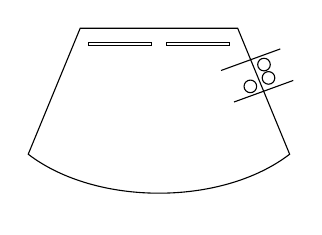
\begin{tikzpicture}[scale=2,baseline={(0,0)},remember picture]
      \draw (0,0) -- (1,0) -- (1.33,-.8) .. controls (0.9,-1.13) and (0.1,-1.13) .. (-0.33,-.8) -- cycle;
      \draw (1.0825,-0.2) -- +(-160:.2) -- +(20:.2);
      \draw (1.165,-0.4) -- +(-160:.2) -- +(20:.2);
      \draw (.25,-.1) coordinate (two) +(-.2,-.01) rectangle +(.2,.01) ;
      \draw [shift={(.75,-.1)}] coordinate (one) +(-.2,-.01) rectangle +(.2,.01);
      \draw (1.0825,-.2) +(-20:.09)   coordinate (three) circle[radius=.04];
      \draw (1.165,-.4) +(90-20:.09)  coordinate (four)  circle[radius=.04];
      \draw (1.165,-.4) +(180-20:.09) coordinate (five)  circle[radius=.04];
    \end{tikzpicture}
    }
    &&&\tikz[remember picture,baseline=0]\path
       (0,0) node[anchor=south west] {}
       ++(0,.2em) coordinate (bta) ++(1ex,3pt) coordinate (btb);
  &\tikz[remember picture,baseline=0]\path
    (0,0) node[anchor=south west] {}
    ++(0,.2em) ++(0,-1pt) coordinate (sta);\\
  &&{\sffamily Før}&Barwin
  &\tikz[BrickRed,remember picture]
    \fill (0,0) coordinate (a)  ++(-.5ex,-.5em)rectangle +(1ex,1em);
  &&\nonactor{BrickRed}\top
  &\nonactor{}\top
  &\nonactor{}\top
  &\nonactor{}\top
  &\nonactor{}\top
  &\nonactor{}\top
  &\anactor{}\top
  &\nonactor{}\top
  &\nonactor{}\top
  &\nonactor{}\top
  &\nonactor{BrickRed}\top
  &\nonactor{}\top
  &\anactor{}\top
  &\anactor{}\top
  &\nonactor{}\top
  &\nonactor{}\top
  &\nonactor{}\top
  &\nonactor{}\top
  &\anactor{}\top
  &\nonactor{}\top
  &\nonactor{}\top
  &\anactor{}\top
  &\nonactor{}\top
  \\
  &&&Stor øl
  &\hspace{1ex}\tikz[OliveGreen,remember picture]
    \fill (0,0) coordinate (b) ++(-.5ex,-.5em) rectangle +(1ex,1em);
  &&\nonactor{}\btm
    &\nonactor{}\btm
      &\nonactor{}\btm
  &\nonactor{}\btm
  &\nonactor{}\btm
  &\nonactor{}\btm
  &\anactor{OliveGreen}\btm
  &\nonactor{}\btm
    &\nonactor{}\btm
      &\nonactor{}\btm
  &\nonactor{}\btm
  &\nonactor{}\btm

  &\anactor{OliveGreen}\btm
  &\anactor{}\btm
  &\nonactor{}\btm
    &\nonactor{}\btm
      &\nonactor{}\btm
  &\nonactor{}\btm
  &\anactor{}\btm
  &\nonactor{}\btm
  &\nonactor{}\btm
  &\anactor{}\btm
  &\nonactor{}\btm
  \\
  &&{\sffamily Under}&3 stole
  &&\tikz[Purple,remember picture]
     \fill (0,0) coordinate (c) ++(-.5ex,-.5em) rectangle +(1ex,1em);
  &\nonactor{}\tpbt
    &\nonactor{}\tpbt
      &\nonactor{}\tpbt
  &\nonactor{}\tpbt
  &\nonactor{}\tpbt
  &\nonactor{}\tpbt
  &\anactor{}\tpbt
  &\nonactor{Purple}\tpbt
  &\nonactor{Purple}\tpbt
  &\nonactor{}\tpbt
  &\nonactor{}\tpbt
  &\nonactor{}\tpbt

  &\anactor{}\tpbt
  &\anactor{}\tpbt
  &\nonactor{}\tpbt
    &\nonactor{}\tpbt
      &\nonactor{}\tpbt
  &\nonactor{}\tpbt
  &\anactor{}\tpbt
  &\nonactor{}\tpbt
  &\nonactor{}\tpbt
  &\anactor{}\tpbt
  &\nonactor{}\tpbt\\
  &&{\sffamily Efter}&Barwin
  &\tikz[BrickRed,remember picture]
    \fill (0,0) coordinate (d) ++(-.5ex,-.5em) rectangle +(1ex,1em);
  &  &\nonactor{BrickRed}\top
    &\nonactor{}\top
      &\nonactor{}\top
  &\nonactor{}\top
  &\nonactor{}\top
  &\nonactor{}\top
  &\anactor{}\top
  &\nonactor{}\top
    &\nonactor{}\top
      &\nonactor{}\top
  &\nonactor{BrickRed}\top
  &\nonactor{}\top
  &\anactor{}\top
  &\anactor{}\top
  &\nonactor{}\top
    &\nonactor{}\top
      &\nonactor{}\top
  &\nonactor{}\top
  &\anactor{}\top
  &\nonactor{}\top
  &\nonactor{}\top
  &\anactor{}\top
  &\nonactor{}\top\\
  &&&Stor øl
  &\hspace{1ex}\tikz[OliveGreen,remember picture]
    \fill (0,0) coordinate (e) ++(-.5ex,-.5em) rectangle +(1ex,1em);
  &&\nonactor{}\btm
    &\nonactor{}\btm
      &\nonactor{}\btm
  &\nonactor{}\btm
  &\nonactor{}\btm
  &\nonactor{}\btm
  &\anactor{OliveGreen}\btm
  &\nonactor{}\btm
    &\nonactor{}\btm
      &\nonactor{}\btm
  &\nonactor{}\btm
  &\nonactor{}\btm
  &\anactor{OliveGreen}\btm
  &\anactor{}\btm
  &\nonactor{}\btm
    &\nonactor{}\btm
      &\nonactor{}\btm
  &\nonactor{}\btm
  &\anactor{}\btm
  &\nonactor{}\btm
  &\nonactor{}\btm
  &\anactor{}{\btm}
  &\nonactor{}\btm    \begin{tikzpicture}[overlay,remember picture]
      \draw[BrickRed] (one) |- (bta)[anchor=south east] -| (d);
      \draw[BrickRed] (two) |- (bta)[anchor=south east] -| (d);
      \draw[Purple] (three) |- (sta);
      \draw[Purple] (four)  |- (sta);
      \draw[Purple] (five)  |- (sta);
      \draw[Purple] (sta) -| (c);
    \end{tikzpicture}
\\
    \midrule
    \multicolumn{4}{l}{(0:20) {\bfseries [FISK] Kun BIO}}&\multicolumn{25}{c}{\bfseries --- FISK ---}\\
    \midrule
    \multicolumn{4}{l}{(4:30) {\bfseries 1.6 Mikrobiologernes Revy}}\\
    \multirow{1}{30ex}{
      \footnotesize
      \begin{itemize}
        \item kanon mm. ind efter "acrobatic"
        \item Anders og Søren Skifter tilbage her
      \end{itemize}
    }
  &
    &&&\tikz[remember picture] \path (0,0) coordinate (tone) ++(0,-2pt) coordinate (ttwo)  ++(0,-2pt) coordinate (tthree) ++(0,-2pt) coordinate (tfour) ++(0,-2pt) coordinate (tfive);\\
    &\multirow{1}{*}{
    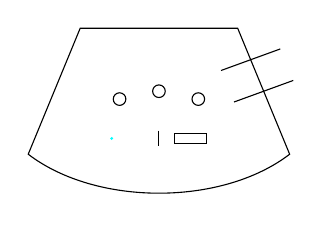
\begin{tikzpicture}[scale=2,baseline={(0,0)},remember picture]
      \draw (0,0) -- (1,0) -- (1.33,-.8) .. controls (0.9,-1.13) and (0.1,-1.13) .. (-0.33,-.8) -- cycle;
      \draw (1.0825,-0.2) -- +(-160:.2) -- +(20:.2);
      \draw (1.165,-0.4) -- +(-160:.2) -- +(20:.2);
      \draw (.5,-.4)   coordinate (one) circle[radius=.04];
      \draw (.25,-.45)  coordinate (two)  circle[radius=.04];
      \draw (.75,-.45) coordinate (three)  circle[radius=.04];
      \fill[Cyan] (.2,-.7) coordinate (four) circle[radius=.01];
      \draw (.5,-.7) coordinate (five) +(0,.05) -- +(0,-.05);
      \draw (.7,-.7) coordinate (six) +(.1,.03) rectangle +(-.1,-.03);
    \end{tikzpicture}
    }&{\sffamily Før}&Kanon&&\tikz[remember picture] \fill[BrickRed] (0,0) rectangle (1ex,1em) coordinate[pos=.5] (bone);&\nonactor{}\top
  &\nonactor{}\top
  &\anactor{}\top
  &\nonactor{}\top
  &\nonactor{}\top
  &\nonactor{}\top
  &\nonactor{}\top
  &\nonactor{}\top
  &\nonactor{BrickRed}\top
  &\nonactor{}\top
  &\nonactor{}\top
  &\nonactor{}\top
  &\nonactor{}\top
  &\nonactor{}\top
  &\anactor{}\top
  &\nonactor{}\top
  &\nonactor{}\top
  &\nonactor{}\top
  &\nonactor{}\top
  &\nonactor{}\top
  &\anactor{}\top
  &\nonactor{}\top
  &\nonactor{}\top\\
    &&&Ildring&&\hspace{1ex}\tikz[remember picture] \fill[OliveGreen] (0,0) rectangle (1ex,1em) coordinate[pos=.5] (btwo);&\nonactor{}{}
  &\nonactor{}{}
  &\anactor{}{}
  &\nonactor{}{}
  &\nonactor{}{}
  &\nonactor{}{}
  &\nonactor{}{}
  &\nonactor{}{}
  &\nonactor{OliveGreen}{}
  &\nonactor{}{}
  &\nonactor{}{}
  &\nonactor{}{}
  &\nonactor{}{}
  &\nonactor{}{}
  &\anactor{}{}
  &\nonactor{}{}
  &\nonactor{}{}
  &\nonactor{}{}
  &\nonactor{}{}
  &\nonactor{}{}
  &\anactor{}{}
  &\nonactor{}{}
  &\nonactor{}{}\\
    &&&Kop m. vand&&\hspace{2ex}\tikz[remember picture] \fill[Purple] (0,0) rectangle (1ex,1em) coordinate[pos=.5] (bthree);&\nonactor{}{}
  &\nonactor{}{}
  &\anactor{}{}
  &\nonactor{}{}
  &\nonactor{}{}
  &\nonactor{}{}
  &\nonactor{}{}
  &\nonactor{}{}
  &\nonactor{Purple}{}
  &\nonactor{}{}
  &\nonactor{}{}
  &\nonactor{}{}
  &\nonactor{}{}
  &\nonactor{}{}
  &\anactor{}{}
  &\nonactor{}{}
  &\nonactor{}{}
  &\nonactor{}{}
  &\nonactor{}{}
  &\nonactor{}{}
  &\anactor{}{}
  &\nonactor{}{}
  &\nonactor{}{}\\
    &&&3 stole&&\hspace{3ex}\tikz[remember picture] \fill[Cyan] (0,0) rectangle (1ex, 1em) coordinate[pos=.5] (bfour);&\nonactor{}\btm
  &\nonactor{}\btm
  &\anactor{}\btm
  &\nonactor{}\btm
  &\nonactor{Cyan}\btm
  &\nonactor{}\btm
  &\nonactor{}\btm
  &\nonactor{Cyan}\btm
  &\nonactor{}\btm
  &\nonactor{}\btm
  &\nonactor{}\btm
  &\nonactor{}\btm
  &\nonactor{}\btm
  &\nonactor{}\btm
  &\anactor{}\btm
  &\nonactor{}\btm
  &\nonactor{}\btm
  &\nonactor{}\btm
  &\nonactor{}\btm
  &\nonactor{}\btm
  &\anactor{}\btm
  &\nonactor{}\btm
  &\nonactor{}\btm\\
    &&{\sffamily Under}&Kanon&&\tikz[remember picture] \fill[BrickRed] (0,0) rectangle (1ex,1em) coordinate[pos=.5] (bfive);&\nonactor{}\top
  &\nonactor{}\top
  &\anactor{}\top
  &\nonactor{}\top
  &\nonactor{}\top
  &\nonactor{}\top
  &\nonactor{}\top
  &\nonactor{}\top
  &\nonactor{BrickRed}\top
  &\nonactor{}\top
  &\nonactor{}\top
  &\nonactor{}\top
  &\nonactor{}\top
  &\nonactor{}\top
  &\anactor{}\top
  &\nonactor{}\top
  &\nonactor{}\top
  &\nonactor{}\top
  &\nonactor{}\top
  &\nonactor{}\top
  &\anactor{}\top
  &\nonactor{}\top
  &\nonactor{}\top\\
    &&&Ildring&&\hspace{1ex}\tikz[remember picture] \fill[OliveGreen] (0,0) rectangle (1ex,1em) coordinate[pos=.5] (bsix);&\nonactor{}{}
  &\nonactor{}{}
  &\anactor{}{}
  &\nonactor{}{}
  &\nonactor{}{}
  &\nonactor{}{}
  &\nonactor{}{}
  &\nonactor{}{}
  &\nonactor{OliveGreen}{}
  &\nonactor{}{}
  &\nonactor{}{}
  &\nonactor{}{}
  &\nonactor{}{}
  &\nonactor{}{}
  &\anactor{}{}
  &\nonactor{}{}
  &\nonactor{}{}
  &\nonactor{}{}
  &\nonactor{}{}
  &\nonactor{}{}
  &\anactor{}{}
  &\nonactor{}{}
  &\nonactor{}{}\\
    &&&Kop m. vand&&\hspace{2ex}\tikz[remember picture] \fill[Purple] (0,0) rectangle (1ex,1em) coordinate[pos=.5] (bseven);&\nonactor{}{}
  &\nonactor{}{}
  &\anactor{}{}
  &\nonactor{}{}
  &\nonactor{}{}
  &\nonactor{}{}
  &\nonactor{}{}
  &\nonactor{}{}
  &\nonactor{Purple}{}
  &\nonactor{}{}
  &\nonactor{}{}
  &\nonactor{}{}
  &\nonactor{}{}
  &\nonactor{}{}
  &\anactor{}{}
  &\nonactor{}{}
  &\nonactor{}{}
  &\nonactor{}{}
  &\nonactor{}{}
  &\nonactor{}{}
  &\anactor{}{}
  &\nonactor{}{}
  &\nonactor{}{}\\
    &&&2 borde&\tikz[remember picture] \fill[Orange] (0,0) rectangle (1ex,1em) coordinate[pos=.5] (btwelve);&&\nonactor{}\btm
  &\nonactor{}\btm
  &\anactor{}\btm
  &\nonactor{}\btm
  &\nonactor{}\btm
  &\nonactor{}\btm
  &\nonactor{}\btm
  &\nonactor{}\btm
  &\nonactor{}\btm
  &\nonactor{Orange}\btm
  &\nonactor{}\btm
  &\nonactor{}\btm
  &\nonactor{Orange}\btm
  &\nonactor{}\btm
  &\anactor{}\btm
  &\nonactor{}\btm
  &\nonactor{Orange}\btm
  &\nonactor{Orange}\btm
  &\nonactor{}\btm
  &\nonactor{}\btm
  &\anactor{}\btm
  &\nonactor{}\btm
  &\nonactor{}\btm\\
    &&{\sffamily Efter}&Kanon&&\tikz[remember picture] \fill[BrickRed] (0,0) rectangle (1ex,1em) coordinate[pos=.5] (beight);&\nonactor{}\top
  &\nonactor{}\top
  &\anactor{}\top
  &\nonactor{}\top
  &\nonactor{}\top
  &\nonactor{}\top
  &\nonactor{}\top
  &\nonactor{}\top
  &\nonactor{BrickRed}\top
  &\nonactor{}\top
  &\nonactor{}\top
  &\nonactor{}\top
  &\nonactor{}\top
  &\nonactor{}\top
  &\anactor{}\top
  &\nonactor{}\top
  &\nonactor{}\top
  &\nonactor{}\top
  &\nonactor{}\top
  &\nonactor{}\top
  &\anactor{}\top
  &\nonactor{}\top
  &\nonactor{}\top\\
    &&&Ildring&&\hspace{1ex}\tikz[remember picture] \fill[OliveGreen] (0,0) rectangle (1ex,1em) coordinate[pos=.5] (bnine);&\nonactor{}{}
  &\nonactor{}{}
  &\anactor{}{}
  &\nonactor{}{}
  &\nonactor{}{}
  &\nonactor{}{}
  &\nonactor{}{}
  &\nonactor{}{}
  &\nonactor{OliveGreen}{}
  &\nonactor{}{}
  &\nonactor{}{}
  &\nonactor{}{}
  &\nonactor{}{}
  &\nonactor{}{}
  &\anactor{}{}
  &\nonactor{}{}
  &\nonactor{}{}
  &\nonactor{}{}
  &\nonactor{}{}
  &\nonactor{}{}
  &\anactor{}{}
  &\nonactor{}{}
  &\nonactor{}{}\\
    &&&Kop m. vand&&\hspace{2ex}\tikz[remember picture] \fill[Purple] (0,0) rectangle (1ex,1em) coordinate[pos=.5] (bten);&\nonactor{}{}
  &\nonactor{}{}
  &\anactor{}{}
  &\nonactor{}{}
  &\nonactor{}{}
  &\nonactor{}{}
  &\nonactor{}{}
  &\nonactor{}{}
  &\nonactor{Purple}{}
  &\nonactor{}{}
  &\nonactor{}{}
  &\nonactor{}{}
  &\nonactor{}{}
  &\nonactor{}{}
  &\anactor{}{}
  &\nonactor{}{}
  &\nonactor{}{}
  &\nonactor{}{}
  &\nonactor{}{}
  &\nonactor{}{}
  &\anactor{}{}
  &\nonactor{}{}
  &\nonactor{}{}\\
    &&&3 stole&&\hspace{3ex}\tikz[remember picture] \fill[Cyan] (0,0) rectangle (1ex, 1em) coordinate[pos=.5] (beleven);&\nonactor{}\btm
  &\nonactor{}\btm
  &\anactor{}\btm
  &\nonactor{}\btm
  &\nonactor{Cyan}\btm
  &\nonactor{}\btm
  &\nonactor{}\btm
  &\nonactor{Cyan}\btm
  &\nonactor{}\btm
  &\nonactor{}\btm
  &\nonactor{}\btm
  &\nonactor{}\btm
  &\nonactor{}\btm
  &\nonactor{}\btm
  &\anactor{}\btm
  &\nonactor{}\btm
  &\nonactor{}\btm
  &\nonactor{}\btm
  &\nonactor{}\btm
  &\nonactor{}\btm
  &\anactor{}\btm
  &\nonactor{}\btm
  &\nonactor{}\btm
    \begin{tikzpicture}[remember picture, overlay]
      \draw[BrickRed] (six) |- (tfour) -| (beight);
      \draw[OliveGreen] (five) |- (tthree) -| (bnine);
      \draw[Purple] (four) |- (ttwo) -| (bten);
      \draw[Cyan] (one) |- (tone) -| (beleven);
      \draw[Cyan] (two) |- (tone) -| (beleven);
      \draw[Cyan] (three) |- (tone) -| (beleven);
    \end{tikzpicture}
\\
    
    \bottomrule
\end{tabular}
  
  % \bottomrule
\end{document}
%%% Local Variables:
%%% mode: LaTeX
%%% TeX-master: t
%%% End:
